\documentclass{article}

% Numeric citation style, as used by the NeurIPS template.
\PassOptionsToPackage{numbers,compress}{natbib}
\usepackage[preprint]{neurips_2023}

\usepackage[utf8]{inputenc}
\usepackage[T1]{fontenc}
\usepackage{hyperref}
\usepackage{url}
\usepackage{booktabs}
\usepackage{amsfonts}
\usepackage{amsmath}
\usepackage{nicefrac}
\usepackage{microtype}
\usepackage{graphicx}
\usepackage{caption}
\usepackage{float}
\usepackage{xcolor}

\graphicspath{{../reports/figures/}}

% The style file's preprint option prints "Preprint. Under review." This work is
% not under review anywhere, so the notice states only what is true.
\makeatletter
\renewcommand{\@noticestring}{%
  Preprint. Code, data, and the full result tables: \url{https://github.com/ITheClixs/crypto-return-predictability}%
}
\makeatother

\hypersetup{
  colorlinks = true,
  linkcolor  = black,
  citecolor  = black,
  urlcolor   = blue!60!black
}

\newcommand{\rsq}{R^2_{OS}}

\title{On the Out-of-Sample Predictability of\\Short-Horizon Cryptocurrency Returns}

\author{%
  Mehmet Demir Guven \\
  Department of Computer Science \\
  ETH Z\"urich \\
}

\begin{document}

\maketitle

\begin{abstract}
  We ask whether daily cryptocurrency returns can be forecast out of sample well
  enough to survive transaction costs, and we design the study so that the
  question is falsifiable rather than flattering. Three assets, two horizons, and
  six forecasters are evaluated by purged and embargoed walk-forward
  cross-validation over 2020--2026, giving 18 machine-learning settings measured
  against a martingale null. The conclusion turns on a choice of test that the
  applied literature usually makes by default. Diebold--Mariano rejects in favour
  of the random walk in 7 of 18 settings and never in favour of a model, which
  would suggest that learning actively hurts. But the random walk is
  \emph{nested} inside every model considered, and under nesting that statistic
  is biased toward the smaller model. Under the Clark--West correction, 5 of 18
  settings reject the no-predictability null at an uncorrected 5\% level, against
  0.9 expected from a search of that size; 2 survive control of the false
  discovery rate and none survives control of the family-wise error rate. The
  survivors are not usable forecasts: their out-of-sample $\rsq$ against a
  recursive drift benchmark is $-0.0079$ and $+0.0031$, and their net Sharpe
  intervals straddle zero. No setting exhibits significant sign-timing skill,
  which is the property a directional strategy actually trades. The settings
  whose Sharpe intervals exclude zero are disjoint from those surviving
  statistical correction, and every high-Sharpe result in the study is long-only
  exposure in disguise. We report a faint, fragile statistical signal and no
  tradeable one, together with the full apparatus that would have detected either.
\end{abstract}

\section{Introduction}

Claims of accurate cryptocurrency price prediction are abundant and rarely
survive scrutiny. The reported accuracy is usually traceable to one of four
errors, each of which is well documented and each of which is easy to commit
without noticing.

\textbf{Target leakage.} The predicted quantity is a function of contemporaneous
or future information, so the model fits an identity rather than forecasting
\citep{kaufman2012}. Leakage of this kind is now understood to be a leading cause
of irreproducible findings in machine-learning-based science more broadly
\citep{kapoor2023}.

\textbf{Preprocessing leakage.} A scaler, imputer, or feature selector is fit on
the full sample before splitting, so the test distribution informs training.

\textbf{Absent benchmarks.} Accuracy is reported on a price series rather than on
returns. Prices are close to a martingale, so a naive random-walk forecast attains
near-perfect $R^2$; a model that appears to explain 99\% of price variance may
explain none of the return variance, which is the only component that can be
traded \citep{timmermann2004}.

\textbf{Silent multiple testing.} Many model, asset, and horizon combinations are
tried and the best is reported without adjusting the threshold. In the closely
analogous cross-sectional asset-pricing literature, \citet{harvey2016} argue that
conventional significance levels are badly miscalibrated once the size of the
collective search is acknowledged.

This paper is organised so that each of these is either impossible by
construction or measured and reported. The contribution is not a model. It is an
evaluation protocol applied honestly to a question with a commercially attractive
answer, which returns the unattractive one.

A second contribution is methodological, and it changed our own conclusion. The
standard tool for comparing forecast accuracy, the Diebold--Mariano test
\citep{diebold1995}, assumes the competing forecasts are non-nested. The
comparison that the return-predictability literature actually makes---a
conditional model against a random walk---violates that assumption, because
setting the model's slopes to zero recovers the benchmark exactly. Under the null
the larger model must still estimate coefficients that are truly zero, and the
resulting estimation noise inflates its sample mean squared prediction error even
though its population error is identical. Section~\ref{sec:cw} sets this out, and
Section~\ref{sec:results-tests} shows that on our data the correction moves the
verdict from ``nothing predicts, several are significantly worse'' to ``five
settings reject, two survive false-discovery control, none is tradeable.'' Both
statements are defensible from the same forecasts. Only the second is correct.

\section{Related work}

\paragraph{Return predictability and out-of-sample evaluation.}
\citet{welch2008} showed that a long list of equity-premium predictors that
perform well in sample fail to beat a simple historical mean out of sample, and
\citet{campbell2008} formalised the out-of-sample $R^2$ against that benchmark
which we adopt in Section~\ref{sec:r2}. The lesson generalises: in-sample fit is
close to uninformative about forecast value, and the appropriate benchmark is a
naive one estimated recursively rather than with hindsight.

\paragraph{Machine learning in asset pricing.}
\citet{gu2020} conduct a large-scale comparison of machine-learning methods for
equity returns and find measurable but small out-of-sample gains, concentrated in
methods that shrink aggressively. Our model roster is chosen in that spirit:
regularised linear models and a deliberately constrained gradient booster, on the
premise that an unregularised learner in this signal-to-noise regime fits noise
and a null result obtained from an overfit model would be uninformative.

\paragraph{Backtest overfitting.}
\citet{bailey2014pseudo} and \citet{arnott2019} document how repeated backtesting
manufactures apparently significant strategies, and \citet{bailey2014} propose the
deflated Sharpe ratio, which raises the bar in proportion to the number of trials.
\citet{white2000} and \citet{sullivan1999} address the same problem for technical
trading rules through a bootstrap reality check. We adopt the deflated Sharpe
ratio together with explicit control of the false discovery rate and the
family-wise error rate over our grid.

\paragraph{Cryptocurrency market efficiency.}
The empirical record is mixed and appears to be time-varying.
\citet{urquhart2016} reports evidence of inefficiency in early Bitcoin returns;
\citet{nadarajah2017} find that a simple power transformation of the same returns
satisfies efficiency tests, and \citet{tiwari2018} report that Bitcoin is largely
efficient over most of their sample. This literature evaluates statistical
efficiency; it generally does not ask whether any detected dependence survives
transaction costs, which is the question we take up.

\paragraph{Validation for dependent data.}
Purged and embargoed cross-validation is due to \citet{lopezdeprado2018}, and is
the mechanism by which we prevent a training label whose realisation overlaps a
test window from informing the fit.

\section{Data}
\label{sec:data}

We use daily adjusted OHLCV bars from Yahoo Finance for the USD pairs of BTC, ETH,
and SOL. BTC and ETH span 2019-01-01 to 2026-07-18 (2{,}756 bars each); SOL begins
2020-04-10 (2{,}291 bars). Cryptocurrency markets trade every calendar day, so the
bar index is contiguous with no weekend or holiday gaps. We verified this rather
than assuming it, and Section~\ref{sec:cv} shows that the split logic remains
conservative under gaps regardless.

The evaluated out-of-sample window is shorter than the data window because the
first fold consumes 504 bars of training history. Table~\ref{tab:data} gives the
resulting per-setting counts.

\begin{table}[t]
  \centering
  \caption{Evaluated out-of-sample window per setting. Counts are forecasts, not
  trades; the trading rule of Section~\ref{sec:strategy} samples every $h$-th bar.}
  \label{tab:data}
  \small
  \begin{tabular}{llrll}
\toprule
Asset & $h$ (days) & OOS forecasts & First & Last \\
\midrule
BTC & 1 & 2185 & 2020-07-23 & 2026-07-16 \\
BTC & 7 & 2173 & 2020-07-29 & 2026-07-10 \\
ETH & 1 & 2185 & 2020-07-23 & 2026-07-16 \\
ETH & 7 & 2173 & 2020-07-29 & 2026-07-10 \\
SOL & 1 & 1720 & 2021-10-31 & 2026-07-16 \\
SOL & 7 & 1708 & 2021-11-06 & 2026-07-10 \\
\bottomrule
\end{tabular}

\end{table}

Asset selection is not survivorship-free. BTC, ETH, and SOL were chosen in
knowledge of their survival, while many contemporaneous tokens did not survive.
This biases the study toward finding profitable long exposure, which strengthens
rather than weakens a negative result about \emph{predictability}, but would
invalidate any cross-sectional claim. Section~\ref{sec:limitations} returns to it.

\section{Method}

\subsection{Features}

Let $C_t, H_t, L_t, V_t$ denote close, high, low, and volume at bar $t$. Every
feature is a function of information available at or before $t$, and all twelve
are scale-free so that a single model can pool across assets trading at very
different price levels. We use cumulative log returns over
$k \in \{1,5,10,21\}$, realised volatility over $w \in \{10,21\}$, Wilder's RSI
over 14 bars recentred to roughly $[-1,1]$, a price-normalised MACD histogram,
two moving-average ratios, a mean normalised range, and a volume $z$-score:
%
\begin{align}
  r_t^{(k)} &= \log \frac{C_t}{C_{t-k}},
  &
  \sigma_t^{(w)} &= \operatorname{sd}\!\left(r_{t-w+1}^{(1)}, \dots, r_t^{(1)}\right),
  \\[2pt]
  \mathrm{RSI}_t &= 100 - \frac{100}{1 + \bar{U}_t / \bar{D}_t},
  &
  \mathrm{macd}_t &= \frac{M_t - S_t}{C_t},
  \\[2pt]
  \mathrm{ma}_t &= \log \frac{\mathrm{SMA}_7(C)_t}{\mathrm{SMA}_{21}(C)_t},
  &
  \mathrm{dist}_t &= \log \frac{C_t}{\mathrm{SMA}_{50}(C)_t},
  \\[2pt]
  \mathrm{range}_t &= \frac{1}{14}\sum_{i=0}^{13} \frac{H_{t-i} - L_{t-i}}{C_{t-i}},
  &
  z_t &= \frac{\log(1+V_t) - \mu_t^{(21)}}{s_t^{(21)}},
\end{align}
%
where $\bar U$ and $\bar D$ are exponentially smoothed gains and losses with
$\alpha = 1/14$, and $M_t = \mathrm{EMA}_{12}(C)_t - \mathrm{EMA}_{26}(C)_t$ with
$S_t = \mathrm{EMA}_9(M)_t$. The longest warm-up is 50 bars; rows with any
undefined feature are dropped.

The absence of look-ahead is enforced by a test rather than by inspection: future
bars are perturbed and every feature value at or before $t$ is asserted unchanged.
This catches an accidental centred window, a sign error in a shift, or a
non-causal smoother, none of which is reliably visible when reading code.

\subsection{Prediction target}

The label attached to a decision made at $t$ is the return realised over
$(t, t+h]$:
%
\begin{equation}
  y_t^{(h)} = \log \frac{C_{t+h}}{C_t}.
\end{equation}
%
The final $h$ rows have no label. We retain them with features and a missing
target, because that is exactly the state a live forecaster occupies on the most
recent bar, and we exclude them from fitting and scoring.

\subsection{Purged, embargoed walk-forward validation}
\label{sec:cv}

Ordinary $k$-fold cross-validation shuffles time and trains on the future. A plain
chronological split is also insufficient: because $y_t^{(h)}$ resolves at $t+h$, a
training row close to the test block carries a label whose realisation overlaps
the test window. Following \citet{lopezdeprado2018}, we purge the $h$ rows before
each test block and impose a further embargo of $e$ bars. Writing $\mathcal{T}_k$
and $\mathcal{V}_k$ for the train and test index sets of fold $k$, every fold
satisfies
%
\begin{equation}
  \max(\mathcal{T}_k) + h + e < \min(\mathcal{V}_k).
  \label{eq:purge}
\end{equation}
%
Test blocks tile forward without overlap. We use an expanding window with
$|\mathcal{T}| \ge 504$ bars, $|\mathcal{V}| = 63$ bars, and $e = 5$, giving 35
folds for BTC and ETH and 28 for SOL. Figure~\ref{fig:design} shows the resulting
layout, drawn from the splits the study actually runs.

\begin{figure}[t]
  \centering
  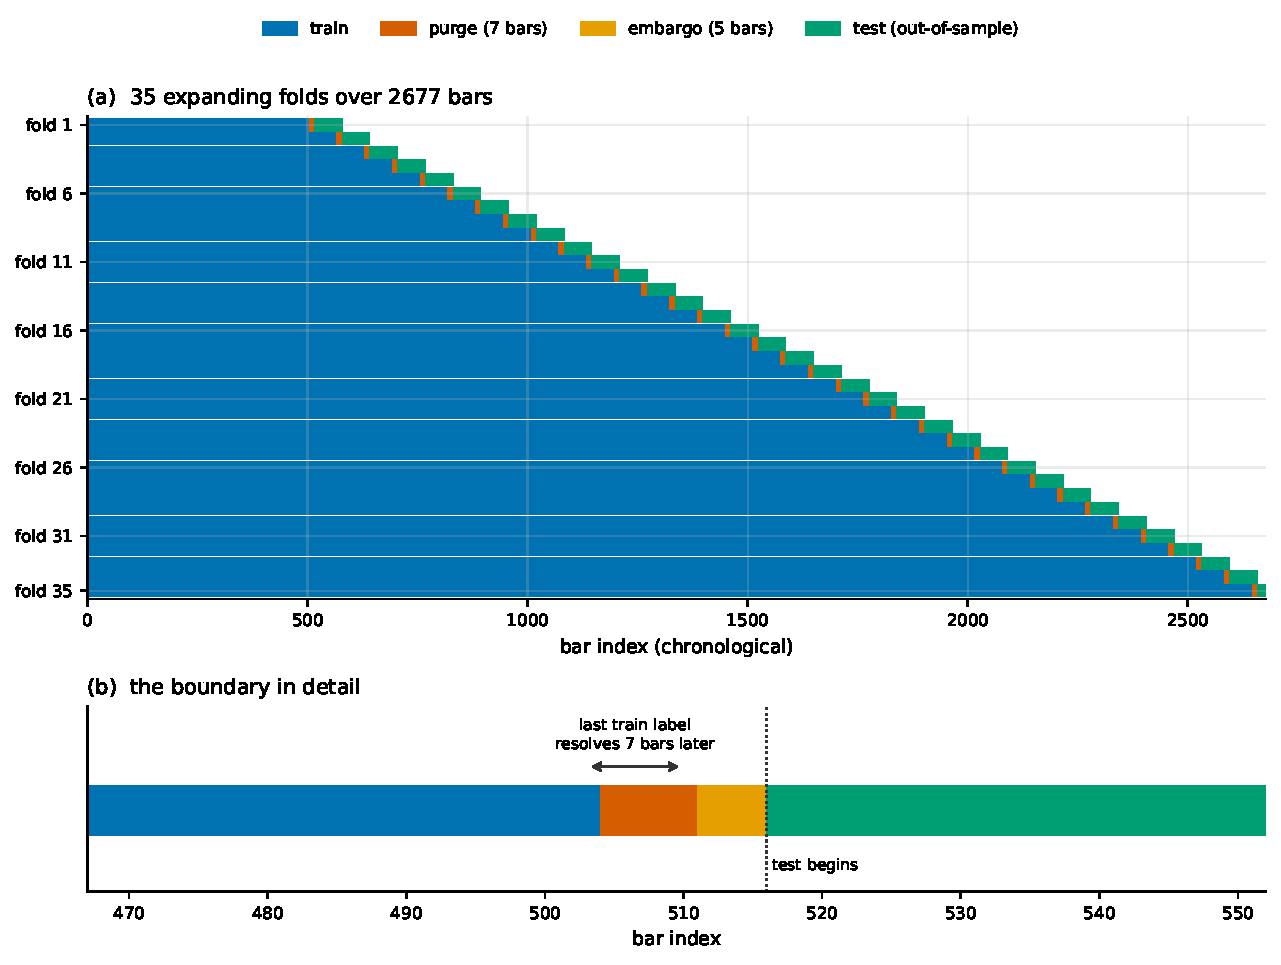
\includegraphics[width=\linewidth]{fig1_design.pdf}
  \caption{The validation design. Panel (a) shows all 35 folds on one timeline;
  panel (b) zooms on a single train/test boundary, where the purge and the embargo
  are individually visible. Equation~\eqref{eq:purge} is what the gap enforces.}
  \label{fig:design}
\end{figure}

Purging is applied by row position, whereas the leak it prevents is a calendar
one. Position-based purging remains valid under missing bars, and conservatively
so: gaps only stretch the timeline, so $h$ positions always span at least $h$
calendar days. We assert this on a synthetic index with a quarter of its bars
removed.

Two further controls are worth naming because they are commonly missed.
Standardisation is a pipeline step fit inside each fold, so it never sees test
rows. And the gradient booster purges its own early-stopping holdout: without a
gap, the last $h$ rows of its fitting slice carry labels realised inside that
holdout, so early stopping would be tuned on partly observed outcomes. We apply
the same $h$-bar purge one level down, and test it by corrupting exactly those
rows and asserting the fitted model is unchanged.

\subsection{Forecasters}

Three benchmarks and three machine-learning models are refit from scratch on every
fold. The benchmarks are the random walk $\hat{y}_t = 0$, the training-window mean
$\hat{y}_t = \bar{y}_{\mathcal{T}}$, and an AR(1) regression of $y^{(h)}$ on
$r^{(1)}$. The machine-learning models are ridge ($\alpha = 1$), elastic net
($\alpha = 10^{-3}$, $\rho = 0.5$), and XGBoost \citep{chen2016} with depth 3,
learning rate $0.03$, subsampling $0.8$, $\lambda = 1$, and early stopping on the
purged temporal holdout described above. The linear objectives are
%
\begin{equation}
  \hat{\beta}_{\text{ridge}} = \arg\min_{\beta} \lVert y - X\beta \rVert_2^2
  + \alpha \lVert \beta \rVert_2^2,
  \qquad
  \hat{\beta}_{\text{EN}} = \arg\min_{\beta} \frac{1}{2n}\lVert y - X\beta \rVert_2^2
  + \alpha \rho \lVert \beta \rVert_1 + \frac{\alpha(1-\rho)}{2}\lVert \beta \rVert_2^2 .
\end{equation}
%
Every one of the three collapses to the random walk when its slopes are zero. They
are nested extensions of the benchmark, which Section~\ref{sec:cw} shows is not a
detail of presentation.

\subsection{Trading rule and transaction costs}
\label{sec:strategy}

Forecasts become unit positions on a non-overlapping schedule: one decision every
$h$ bars, held to the next. Sampling every $h$-th bar prevents the same $h$-day
return being counted $h$ times. Costs are charged on turnover, so reversing a
position pays for two sides:
%
\begin{equation}
  w_t = \operatorname{sign}(\hat{y}_t) \in \{-1, 0, +1\},
  \qquad
  \tau_t = |w_t - w_{t-1}|,
  \qquad
  \pi_t = w_t\!\left(e^{y_t^{(h)}} - 1\right) - \tau_t c,
\end{equation}
%
with $c = 17$ basis points per side (10 bp taker fee, 5 bp slippage, 2 bp
half-spread). Equity compounds as $E_T = \prod_{t \le T}(1 + \pi_t)$ from unity.

Because decisions are taken every $h$ bars, the Sharpe ratio annualises at $365/h$
rather than at 365. Using the latter inflates a seven-day strategy's Sharpe by a
factor of $\sqrt{7} \approx 2.6$.

The schedule admits $h$ start offsets and nothing distinguishes them. We therefore
run every strategy on all $h$ and report the spread, which
Section~\ref{sec:robustness} shows is not a formality.

An always-long reference is computed on the same schedule with the same cost
model, so that a forecaster whose only achievement is holding the asset can be
recognised as such.

\subsection{Out-of-sample $\rsq$}
\label{sec:r2}

We report the Campbell--Thompson form \citep{campbell2008}, whose denominator is
the squared error of a genuine ex-ante benchmark forecast rather than of the
realised mean of the evaluation window:
%
\begin{equation}
  \rsq = 1 - \frac{\sum_t (y_t - \hat{y}_t)^2}{\sum_t (y_t - \hat{y}^{\,b}_t)^2},
\end{equation}
%
with $\hat{y}^{\,b}$ the recursively estimated historical mean. That benchmark
scores exactly zero against itself, which serves as a wiring check on the metric.
The alternative denominator $\sum_t (y_t - \bar{y})^2$ uses a quantity unknowable
in advance and flatters the benchmark; we compute it as a cross-check but do not
quote it.

\subsection{Diebold--Mariano and the nested-model problem}

For loss differential $d_t = L(e^m_t) - L(e^b_t)$ under squared-error loss, the
Diebold--Mariano statistic \citep{diebold1995} is $\mathrm{DM} = \bar{d}/\sqrt{\hat{V}/n}$
with $\hat V$ a Newey--West long-run variance \citep{newey1987} truncated at $h-1$
Bartlett lags, appropriate because $h$-step forecast errors follow an MA($h-1$):
%
\begin{equation}
  \hat{V} = \hat{\gamma}_0 + 2\sum_{k=1}^{h-1}\left(1 - \frac{k}{h}\right)\hat{\gamma}_k,
  \qquad
  \hat{\gamma}_k = \frac{1}{n}\sum_{t=k+1}^{n}(d_t - \bar{d})(d_{t-k} - \bar{d}).
\end{equation}
%
The $1/n$ normalisation applies to every autocovariance including the lagged ones.
This is deliberate: the Bartlett weights guarantee $\hat V \ge 0$ only under that
normalisation, and the more intuitive $1/(n-k)$ can drive a weighted sum negative
in small samples. We apply the Harvey--Leybourne--Newbold small-sample correction
\citep{harvey1997},
$\mathrm{DM}^{\ast} = \mathrm{DM}\sqrt{(n + 1 - 2h + h(h-1)/n)/n}$, against a
$t_{n-1}$ reference. A negative statistic favours the model, and the test is
two-sided because the null is equal accuracy and a model can be significantly
worse.

\subsection{Clark--West}
\label{sec:cw}

Because the random walk is nested in each of our models, Diebold--Mariano is
undersized as a test of predictability: under the null the larger model pays
sample mean squared prediction error to estimate coefficients that are truly zero,
and the test reads that cost as evidence for the benchmark. \citet{clark2007}
subtract the term explicitly. With $\hat{y}^{\,b}$ the nested benchmark and
$\hat{y}^{\,m}$ the larger model,
%
\begin{equation}
  \hat{f}_t = \left(y_t - \hat{y}^{\,b}_t\right)^2
  - \left[\left(y_t - \hat{y}^{\,m}_t\right)^2
  - \left(\hat{y}^{\,b}_t - \hat{y}^{\,m}_t\right)^2\right],
\end{equation}
%
and $\bar{f}/\sqrt{\hat{V}_f/n}$ is referred to a standard normal, one-sided. A
\emph{positive} statistic favours the model, opposite to Diebold--Mariano, which
is reason enough never to report either $p$-value without its statistic.

We verify the bias by simulation rather than asserting it. Over 200 replications
in which the larger model forecasts pure noise, so that the null holds by
construction, the mean Diebold--Mariano statistic is positive and it rejects in
favour of the benchmark far above the nominal rate, while Clark--West remains
centred on zero and holds its size.

\subsection{Sign timing}

A model can be poor at magnitude and useful at direction, which is all a sign
strategy requires. \citet{pesaran1992} test independence between the sign of the
forecast and the sign of the outcome. With $P$ the hit rate, $P_y$ and $P_x$ the
proportions of positive outcomes and forecasts, and
$P_{\ast} = P_y P_x + (1-P_y)(1-P_x)$,
%
\begin{equation}
  S = \frac{P - P_{\ast}}
  {\sqrt{\widehat{\operatorname{var}}(P) - \widehat{\operatorname{var}}(P_{\ast})}}
  \;\xrightarrow{\;d\;}\; \mathcal{N}(0,1),
  \qquad
  \widehat{\operatorname{var}}(P) = \frac{P_{\ast}(1 - P_{\ast})}{n},
\end{equation}
\begin{equation}
  \widehat{\operatorname{var}}(P_{\ast}) = \frac{(2P_y-1)^2 P_x (1-P_x)}{n}
  + \frac{(2P_x-1)^2 P_y (1-P_y)}{n}
  + \frac{4 P_y P_x (1-P_y)(1-P_x)}{n^2}.
\end{equation}
%
A positive statistic indicates sign-timing skill and a negative one indicates a
reliably wrong-way forecast. The statistic is undefined when the forecast never
changes sign, which is precisely the case for the always-long drift models, and we
report it as missing rather than as a number.

\subsection{Sharpe ratio, deflation, and interval estimates}

Sharpe ratios are noisy in short samples \citep{lo2002} and inflated by selection.
The probabilistic Sharpe ratio \citep{bailey2014} gives the probability that the
true Sharpe exceeds a benchmark $\mathrm{SR}^{\ast}$, correcting for sample length,
skewness $\gamma_3$, and kurtosis $\gamma_4$:
%
\begin{equation}
  \widehat{\mathrm{PSR}}(\mathrm{SR}^{\ast}) = \Phi\!\left[
  \frac{(\widehat{\mathrm{SR}} - \mathrm{SR}^{\ast})\sqrt{n-1}}
  {\sqrt{1 - \gamma_3 \widehat{\mathrm{SR}}
  + \frac{\gamma_4 - 1}{4}\widehat{\mathrm{SR}}^{2}}}\right].
\end{equation}
%
The deflated Sharpe ratio sets $\mathrm{SR}^{\ast}$ to the expected maximum across
$N$ trials, so the bar rises with the size of the search:
%
\begin{equation}
  \mathbb{E}\!\left[\max_{i \le N} \mathrm{SR}_i\right] \approx
  \sigma_{\mathrm{SR}}\!\left[(1-\gamma)\,\Phi^{-1}\!\left(1 - \tfrac{1}{N}\right)
  + \gamma\,\Phi^{-1}\!\left(1 - \tfrac{1}{Ne}\right)\right],
\end{equation}
%
with $\gamma$ the Euler--Mascheroni constant. Here $N$ is the number of models
raced within one asset--horizon, which is a floor on the true search; the reported
deflated Sharpe is therefore an upper bound and we label it as such. Confidence
intervals come from a circular block bootstrap \citep{politis1994} with block
length $\lfloor n^{1/3} \rceil$ and 500 resamples, reported as percentile
intervals.

\subsection{Multiple testing}

Eighteen settings tested at the 5\% level produce $0.05 \times 18 = 0.9$
rejections from noise alone. We therefore report raw counts alongside two
adjustments of the Clark--West $p$-values over the family of 18. Holm--Bonferroni
\citep{holm1979} controls the family-wise error rate and Benjamini--Hochberg
\citep{benjamini1995} the false discovery rate:
%
\begin{equation}
  p^{\mathrm{Holm}}_{(i)} = \max_{j \le i}\, \min\!\left\{(m - j + 1)\,p_{(j)},\, 1\right\},
  \qquad
  p^{\mathrm{BH}}_{(i)} = \min_{j \ge i}\, \min\!\left\{\tfrac{m}{j}\,p_{(j)},\, 1\right\}.
\end{equation}
%
Benchmarks are excluded from the family: they are the null being tested against,
not candidates in the search.

\section{Results}

\subsection{Point accuracy}

Out-of-sample $\rsq$ is negative in 16 of 18 machine-learning settings, from
$-0.0908$ (ETH, $h=7$, ridge) to $+0.0031$ (BTC, $h=1$, elastic net). Rank
information coefficients lie between $-0.080$ and $+0.053$. Figure~\ref{fig:r2}
gives the full surface and Table~\ref{tab:accuracy} the underlying numbers.

\begin{figure}[t]
  \centering
  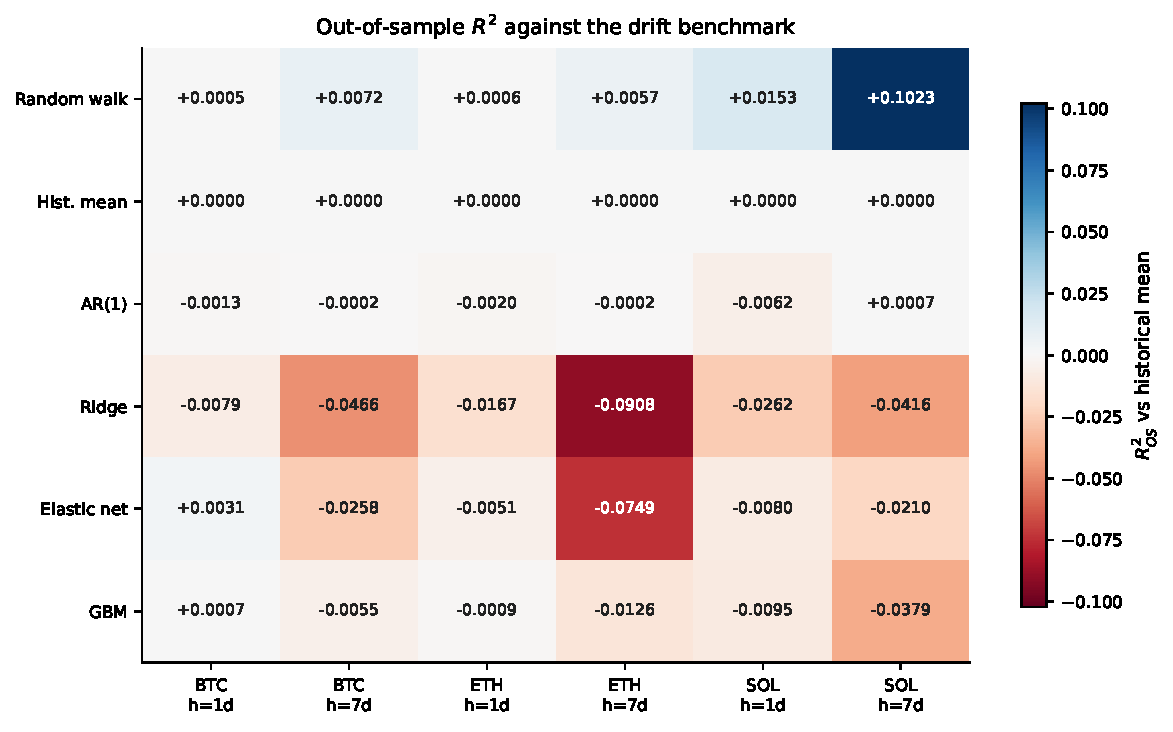
\includegraphics[width=0.86\linewidth]{fig2_r2.pdf}
  \caption{Out-of-sample $\rsq$ against the drift benchmark. Red is worse than an
  ex-ante historical-mean forecast, blue better. The benchmark row is exactly zero
  by construction, which fixes the scale.}
  \label{fig:r2}
\end{figure}

That ridge attains $\mathrm{CW} = +2.62$ with $p = 0.004$ on BTC at $h=1$ while
its $\rsq$ is $-0.0079$ is not a contradiction. Clark--West asks whether the
\emph{population} mean squared prediction error is lower, and a model can satisfy
that while its own parameter-estimation noise leaves the realised forecast worse
than a constant. It is evidence of a weak signal, not of a usable forecast.

\subsection{Predictive accuracy against the random walk}
\label{sec:results-tests}

\begin{figure}[t]
  \centering
  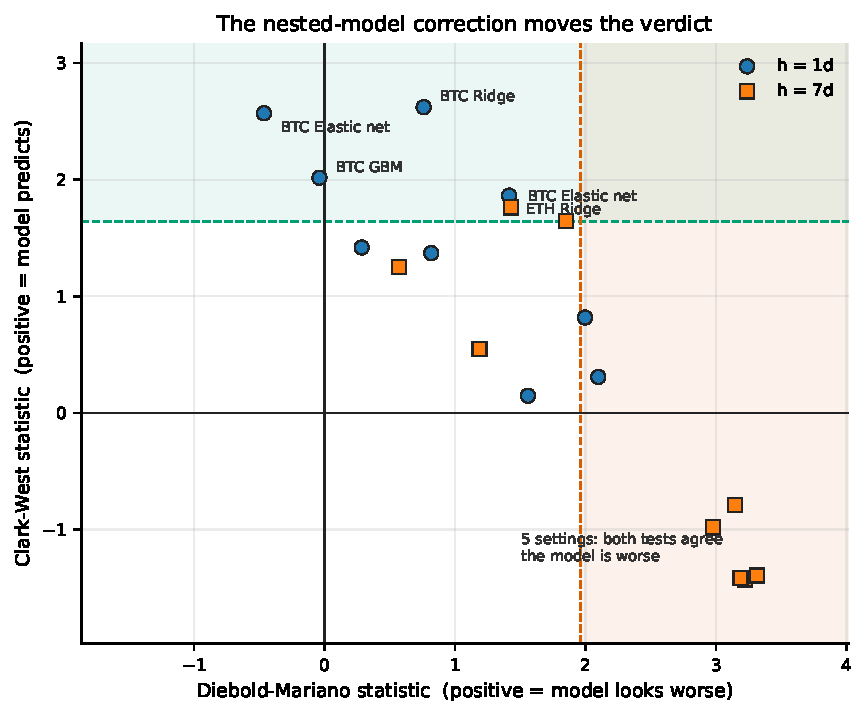
\includegraphics[width=0.78\linewidth]{fig4_dm_vs_cw.pdf}
  \caption{Every setting placed by its Diebold--Mariano statistic against its
  Clark--West statistic. The shaded vertical band marks where DM calls the model
  significantly worse; the horizontal band marks where Clark--West rejects
  no-predictability. Points falling in both are the settings DM misreads. The two
  tests disagree by construction under nesting, and the scatter shows the
  disagreement rather than asserting it.}
  \label{fig:dmcw}
\end{figure}

The two tests disagree, and the disagreement is the finding.
Table~\ref{tab:inference} summarises. Under Diebold--Mariano the conclusion would
be that machine learning is actively harmful here: no setting beats the random
walk and seven lose to it significantly. Under the test valid for nested models,
five settings reject the null of no predictability. Both numbers derive from
identical forecasts.

Ordered by $p$-value the five are BTC ridge ($p = 0.004$), BTC elastic net
($0.005$), BTC GBM ($0.022$), and ETH ridge ($0.031$), all at $h = 1$, together
with BTC elastic net at $h = 7$ ($0.039$). Four of the five are BTC and four are
at the one-day horizon. That concentration is consistent with a weak short-horizon
effect in the most liquid asset, and equally consistent with chance over a search
of this size.

\begin{table}[t]
  \centering
  \caption{Outcome of each test and correction across the 18 machine-learning
  settings. Direction is required, not merely significance: a Diebold--Mariano
  rejection is attributed to whichever side the statistic's sign favours.}
  \label{tab:inference}
  \small
  \begin{tabular}{lr}
\toprule
Criterion & Settings \\
\midrule
Diebold--Mariano, favours model & 0 / 18 \\
Diebold--Mariano, favours benchmark & 7 / 18 \\
Clark--West, uncorrected & 5 / 18 \\
Clark--West, Benjamini--Hochberg & 2 / 18 \\
Clark--West, Holm--Bonferroni & 0 / 18 \\
Pesaran--Timmermann, sign skill & 0 / 18 \\
Pesaran--Timmermann, anti-predictive & 2 / 18 \\
Net Sharpe interval excludes zero & 2 / 18 \\
\addlinespace
\emph{Expected by chance at $\alpha=0.05$} & 0.9 / 18 \\
\bottomrule
\end{tabular}

\end{table}

\subsection{Multiple testing}

\begin{figure}[t]
  \centering
  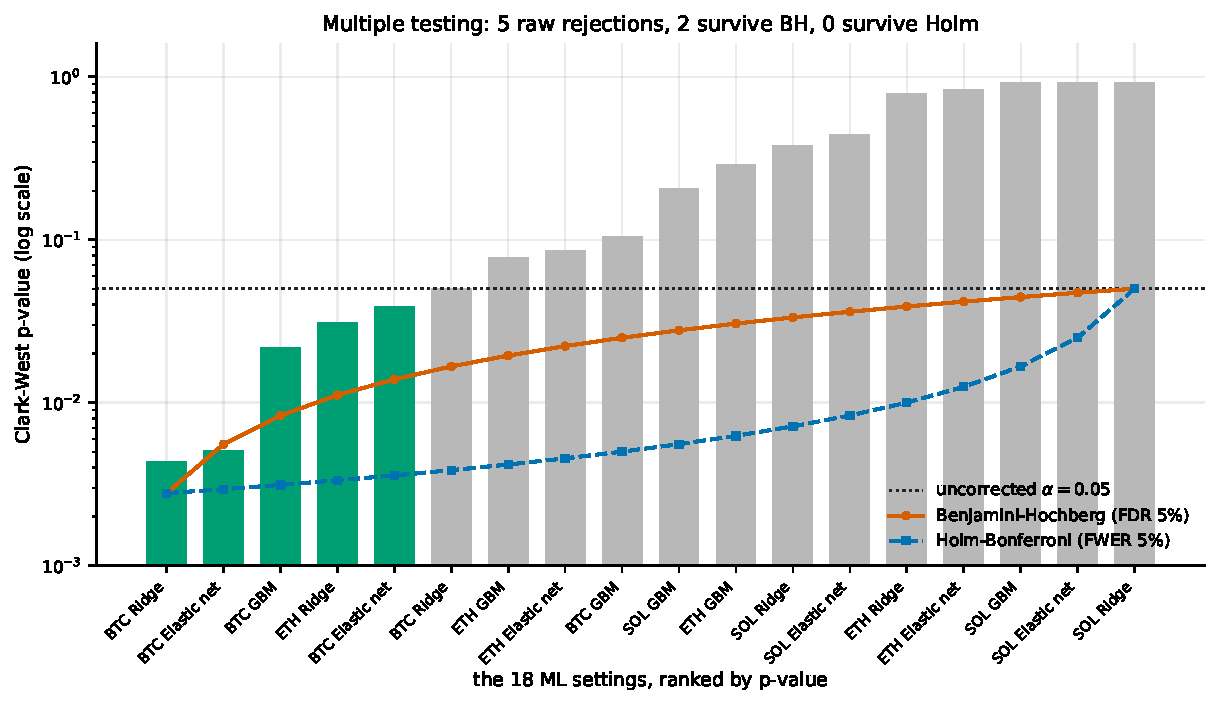
\includegraphics[width=0.86\linewidth]{fig5_multiple_testing.pdf}
  \caption{The 18 Clark--West $p$-values ranked against the Holm--Bonferroni and
  Benjamini--Hochberg thresholds, on a logarithmic scale because the entire
  decision occurs below $p = 0.05$. A bar must fall below a line to be rejected by
  that procedure. Testing 18 settings at the 5\% level is expected to yield 0.9
  rejections from noise alone.}
  \label{fig:mt}
\end{figure}

Controlling the false discovery rate at 5\% leaves BTC ridge and BTC elastic net
at $h=1$, both with $p^{\mathrm{BH}} = 0.046$, marginally under the line.
Controlling the family-wise error rate leaves nothing: the smallest raw $p$-value,
$0.0044$, does not clear the Holm threshold of $0.05/18 = 0.0028$
(Figure~\ref{fig:mt}). The evidence for predictability is real but marginal, and
would not survive a stricter reader.

\subsection{Sign timing}

\begin{figure}[t]
  \centering
  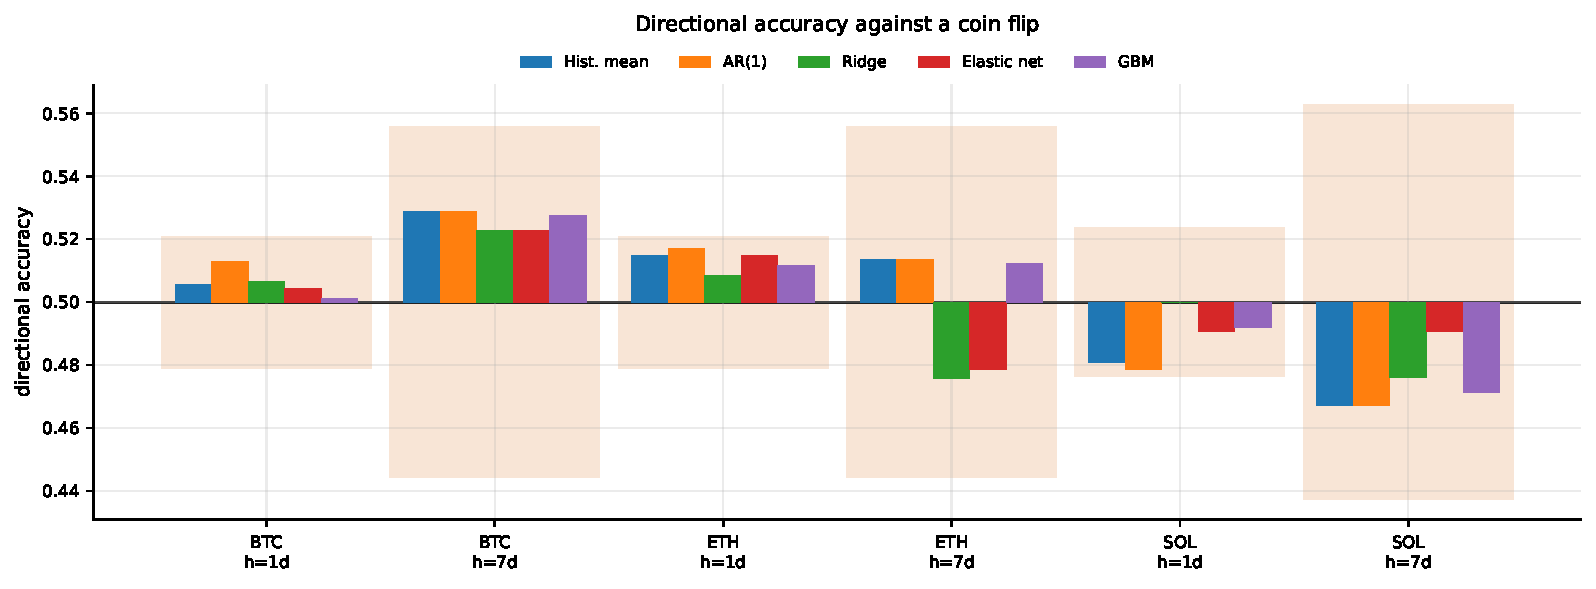
\includegraphics[width=0.92\linewidth]{fig3_diracc.pdf}
  \caption{Directional accuracy against the band a fair coin would occupy. The
  band uses the effective sample size $n/h$: consecutive $h$-day forecasts are
  built from overlapping windows, and treating each as independent would shrink
  the band by $\sqrt{h}$ and manufacture significance.}
  \label{fig:diracc}
\end{figure}

Directional accuracy spans $0.471$ to $0.528$ and every setting lies inside its
coin-flip band (Figure~\ref{fig:diracc}). No setting exhibits significant
sign-timing skill. Two are significantly \emph{anti}-predictive: ETH ridge and ETH
elastic net at $h=7$ give $S = -3.29$ and $S = -3.33$, both $p \approx 0.001$,
with hit rates of $0.476$ and $0.479$.

Those two illustrate why we never report a bare $p$-value. Presented as
``$p = 0.001$'' alone they read as the strongest findings in the study. They are
among the worst.

\subsection{Economic performance}

\begin{figure}[t]
  \centering
  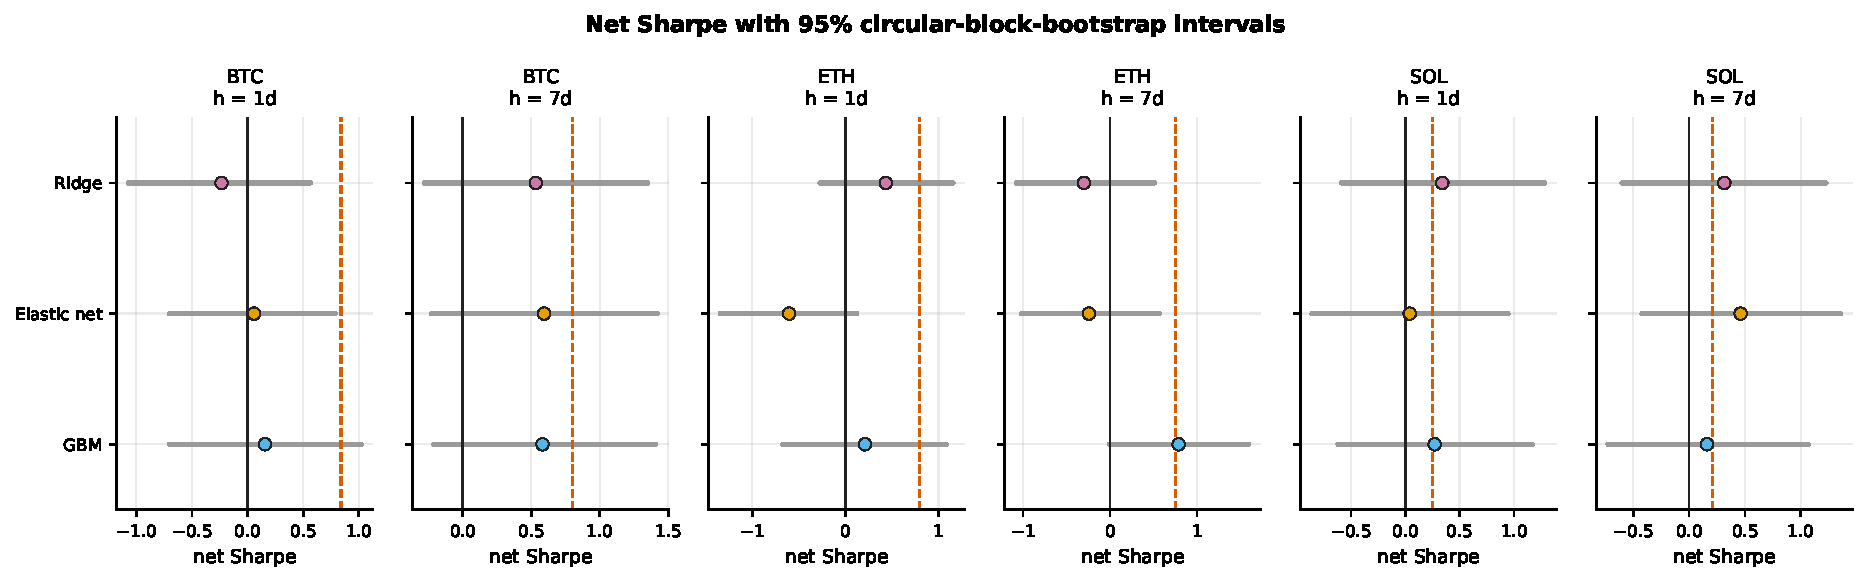
\includegraphics[width=\linewidth]{fig7_sharpe.pdf}
  \caption{Net Sharpe with 95\% circular-block-bootstrap intervals. The dashed
  line marks buy-and-hold on the same schedule and cost model. Intervals excluding
  zero are highlighted.}
  \label{fig:sharpe}
\end{figure}

Two of 18 settings have a net Sharpe whose interval excludes zero, both gradient
boosting on ETH: $0.91$ with interval $[0.00, 1.74]$ at $h=1$, and $0.92$ with
$[0.02, 1.80]$ at $h=7$. Both intervals begin essentially at zero. Neither setting
appears among the two surviving Benjamini--Hochberg correction, and neither of
those two has an interval excluding zero.

The statistical winners and the economic winners are therefore disjoint. Two
unrelated groups of survivors drawn from one search is the signature of noise: if
a genuine short-horizon effect existed and were tradeable, the settings that
detect it and the settings that profit from it ought to overlap.

Six of 18 settings out-Sharpe buy-and-hold on the point estimate, the weakest form
of that claim given that every interval contains zero. Meanwhile the
historical-mean forecaster attains Sharpe ratios of $0.84$, $0.80$, and $0.25$
across the three assets, which is impressive until one observes that it makes
exactly one position change. It predicts a positive drift, hence is always long,
and its net returns are numerically identical to buy-and-hold asset by asset and
horizon by horizon. We carry buy-and-hold as an explicit row in
Table~\ref{tab:performance} so that this cannot be mistaken for model performance.

Maximum drawdowns range from $-55\%$ to $-99\%$ across the machine-learning
settings. This is a property of the position sizing rather than of any model: unit
leverage reversing direction on roughly 70\% annualised volatility carries a large
variance drag, so the geometric return sits well below the arithmetic one.
Buy-and-hold itself draws down between $76\%$ and $96\%$ over the same window.

\subsection{Robustness to the trading schedule}
\label{sec:robustness}

\begin{figure}[t]
  \centering
  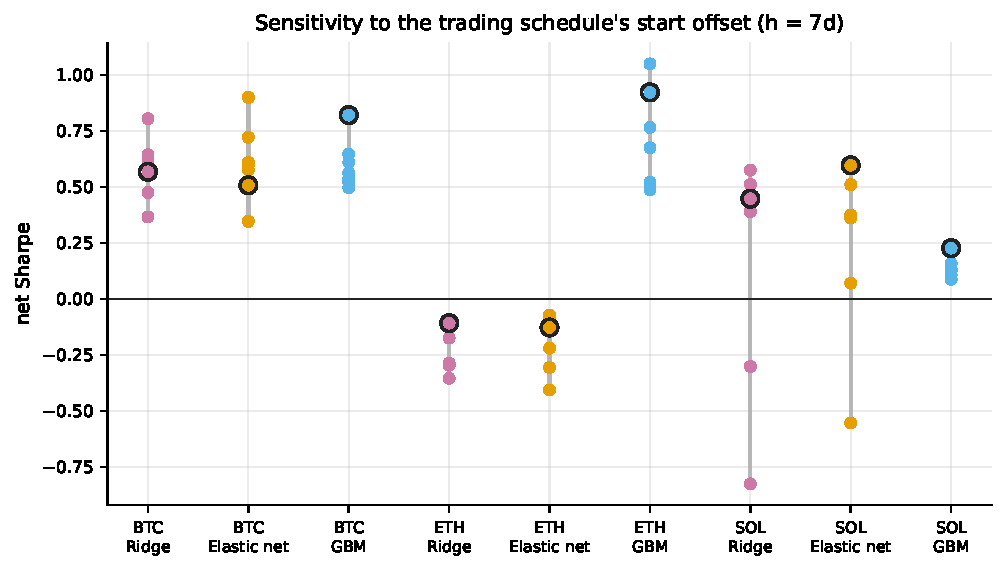
\includegraphics[width=0.92\linewidth]{fig8_phase.pdf}
  \caption{Net Sharpe on each of the $h$ possible start offsets of the trading
  schedule at $h = 7$. The circled point is the offset the results table reports;
  nothing privileges it.}
  \label{fig:phase}
\end{figure}

Sampling every $h$-th bar leaves $h$ schedules and nothing privileges the one
starting at the first bar. At $h=7$ the spread is substantial: SOL ridge reports a
Sharpe of $0.45$ drawn from a distribution running from $-0.83$ to $0.57$, and SOL
elastic net reports $0.60$ from a range of $[-0.55, 0.60]$. The headline number is
in part a property of where sampling happened to begin. A study reporting a
single-offset Sharpe at a multi-day horizon without this check is reporting one
draw and calling it an estimate.

\section{Discussion}

Three points seem worth carrying forward.

\textbf{The choice of test changed the answer.} Diebold--Mariano is the default in
applied forecast comparison, and it is the wrong default whenever the benchmark is
nested, which it is in nearly every return-predictability study that pits a model
against a random walk. The difference here is not cosmetic: ``0 of 18, and 7
significantly worse'' versus ``5 of 18 reject.'' A reader shown only the first
would conclude the models are harmful; a reader shown only the second, without the
multiple-testing correction, would conclude something was found. Neither is the
result.

\textbf{Statistical significance and economic value separated cleanly.} The
settings that reject no-predictability have negative or near-zero out-of-sample
$\rsq$ and Sharpe intervals straddling zero, while the settings that make money do
not reject. This is what a correctly specified null looks like when it is true,
and it is more informative than either group appearing alone.

\textbf{Most apparent performance was exposure.} The highest Sharpe ratios in the
study belong to a forecaster that never changes its mind. An evaluation omitting a
buy-and-hold reference would have credited a drift model with skill it does not
possess. This is a mundane failure mode and, we suspect, a common one.

The result is consistent with weak-form efficiency at daily frequency for
large-capitalisation cryptocurrencies over this period, net of realistic costs
\citep{fama1970}. It does not establish that no cryptocurrency signal exists. It
establishes that this feature set, at these horizons, on these assets, does not
produce one that survives its own error bars.

\section{Limitations}
\label{sec:limitations}

Asset selection is not survivorship-free, as noted in Section~\ref{sec:data}. We
use daily spot bars only, with no order book, funding rates, intraday structure,
or cross-exchange information; short-horizon predictability, if it exists, is more
likely to live at frequencies this data cannot resolve. The feature set is compact
and the model families are three, so richer features or sequence models might
change the picture, though the leakage discipline would not need to change with
them. Short positions are modelled as fully collateralised, returning $-r$ with no
borrow cost, margin requirement, or liquidation, which is reasonable for assessing
signal quality and optimistic as an execution model. Costs are a flat per-side
estimate that does not scale with size or volatility. Intervals are percentile
bootstrap rather than BCa, adequate for a reject/do-not-reject reading and mildly
biased for a statistic as asymmetric as the Sharpe ratio. The deflated Sharpe
ratio understates the true search, deflating for the models raced within one
asset--horizon rather than for the whole grid and for the design choices fixed
before the grid was run. Finally, the sample end date is unpinned, so re-running
extends the window; the evaluated window is stamped into the generated report so
that any table can be tied to the data producing it.

\section{Conclusion}

Across 18 model, asset, and horizon combinations evaluated by purged walk-forward
cross-validation from 2020 to 2026, we find a faint statistical signal in BTC at
the one-day horizon that survives false-discovery control and does not survive
family-wise control. It does not convert into a forecast beating an ex-ante drift
estimate, into sign-timing skill, or into a Sharpe ratio distinguishable from zero
after costs. The strategies with the highest Sharpe ratios in the study are
long-only exposure.

The negative result is the deliverable, and it is reported alongside the tests
that would have detected a positive one and the corrections that would have
removed a spurious one.

\paragraph{Reproducibility.} All results, figures, and tables in this paper are
generated by a single command from a public repository, with a test suite of 154
tests covering the leakage guarantees, the statistical formulas against
hand-computed reference values, and the simulation demonstrating the
Diebold--Mariano bias. The tables reproduced here are emitted directly from the
committed results file rather than transcribed.

\bibliographystyle{unsrtnat}
\bibliography{references}

\appendix

\section{Full results}

Table~\ref{tab:accuracy} gives forecast accuracy and all three predictive-accuracy
tests for every model, asset, and horizon. Table~\ref{tab:performance} gives
net-of-cost performance with bootstrap intervals, the phase spread, and both
Sharpe corrections. Entries in bold are significant at the uncorrected 5\% level;
Section~\ref{sec:results-tests} gives the corrected counts, which are what should
be read.

\begin{table}[H]
  \centering
  \caption{Forecast accuracy and predictive-accuracy tests, all settings. Each
  test is reported as statistic $(p)$. DM negative favours the model, CW positive
  favours the model, PT positive indicates sign-timing skill.}
  \label{tab:accuracy}
  \scriptsize
  \begin{tabular}{lrrrrrrr}
\toprule
Model & RMSE & $R^2_{OS}$ & Dir.\ acc. & Rank IC & DM $(p)$ & CW $(p)$ & PT $(p)$ \\
\midrule
\multicolumn{8}{l}{\emph{BTC, $h=1$}} \\
\quad Random walk & 0.0301 & 0.0005 & -- & -- & -- & -- & -- \\
\quad Historical mean & 0.0301 & 0.0000 & 0.506 & 0.002 & +0.18\,(0.860) & +1.03\,(0.152) & -- \\
\quad AR(1) & 0.0301 & -0.0013 & 0.513 & 0.033 & +0.34\,(0.737) & +1.24\,(0.107) & +1.24\,(0.214) \\
\quad Ridge & 0.0302 & -0.0079 & 0.506 & 0.049 & +0.76\,(0.447) & \textbf{+2.62\,(0.004)} & +0.51\,(0.609) \\
\quad Elastic net & 0.0301 & 0.0031 & 0.505 & 0.046 & -0.46\,(0.644) & \textbf{+2.57\,(0.005)} & +0.25\,(0.806) \\
\quad GBM & 0.0301 & 0.0007 & 0.501 & 0.019 & -0.04\,(0.970) & \textbf{+2.02\,(0.022)} & -0.38\,(0.704) \\
\addlinespace
\multicolumn{8}{l}{\emph{BTC, $h=7$}} \\
\quad Random walk & 0.0804 & 0.0072 & -- & -- & -- & -- & -- \\
\quad Historical mean & 0.0807 & 0.0000 & 0.529 & -0.018 & +0.41\,(0.685) & +1.01\,(0.156) & -- \\
\quad AR(1) & 0.0807 & -0.0002 & 0.529 & -0.023 & +0.42\,(0.675) & +1.00\,(0.159) & -- \\
\quad Ridge & 0.0825 & -0.0466 & 0.523 & 0.044 & +1.85\,(0.064) & +1.64\,(0.050) & +1.41\,(0.159) \\
\quad Elastic net & 0.0817 & -0.0258 & 0.523 & 0.043 & +1.43\,(0.152) & \textbf{+1.76\,(0.039)} & +1.24\,(0.217) \\
\quad GBM & 0.0809 & -0.0055 & 0.528 & 0.032 & +0.57\,(0.569) & +1.25\,(0.105) & +0.74\,(0.459) \\
\addlinespace
\multicolumn{8}{l}{\emph{ETH, $h=1$}} \\
\quad Random walk & 0.0407 & 0.0006 & -- & -- & -- & -- & -- \\
\quad Historical mean & 0.0407 & 0.0000 & 0.515 & 0.019 & +0.25\,(0.806) & +0.81\,(0.209) & -- \\
\quad AR(1) & 0.0408 & -0.0020 & 0.517 & 0.036 & +0.47\,(0.639) & +1.16\,(0.124) & +0.96\,(0.340) \\
\quad Ridge & 0.0411 & -0.0167 & 0.509 & 0.053 & +1.42\,(0.157) & \textbf{+1.86\,(0.031)} & +0.54\,(0.588) \\
\quad Elastic net & 0.0409 & -0.0051 & 0.515 & 0.040 & +0.82\,(0.413) & +1.37\,(0.085) & +1.02\,(0.308) \\
\quad GBM & 0.0408 & -0.0009 & 0.512 & 0.021 & +0.29\,(0.775) & +1.42\,(0.078) & -0.30\,(0.766) \\
\addlinespace
\multicolumn{8}{l}{\emph{ETH, $h=7$}} \\
\quad Random walk & 0.1073 & 0.0057 & -- & -- & -- & -- & -- \\
\quad Historical mean & 0.1076 & 0.0000 & 0.514 & 0.039 & +0.39\,(0.697) & +0.89\,(0.188) & -- \\
\quad AR(1) & 0.1076 & -0.0002 & 0.514 & 0.033 & +0.40\,(0.686) & +0.87\,(0.191) & -- \\
\quad Ridge & 0.1123 & -0.0908 & 0.476 & -0.047 & \textbf{+3.15\,(0.002)} & -0.79\,(0.785) & \textbf{-3.29\,(0.001)} \\
\quad Elastic net & 0.1115 & -0.0749 & 0.479 & -0.052 & \textbf{+2.98\,(0.003)} & -0.98\,(0.837) & \textbf{-3.33\,(0.001)} \\
\quad GBM & 0.1082 & -0.0126 & 0.512 & -0.042 & +1.19\,(0.235) & +0.55\,(0.291) & +0.21\,(0.835) \\
\addlinespace
\multicolumn{8}{l}{\emph{SOL, $h=1$}} \\
\quad Random walk & 0.0498 & 0.0153 & -- & -- & -- & -- & -- \\
\quad Historical mean & 0.0502 & 0.0000 & 0.481 & -0.029 & \textbf{+3.01\,(0.003)} & -1.23\,(0.891) & -- \\
\quad AR(1) & 0.0504 & -0.0062 & 0.478 & -0.007 & \textbf{+2.39\,(0.017)} & -0.77\,(0.779) & -0.81\,(0.415) \\
\quad Ridge & 0.0509 & -0.0262 & 0.500 & 0.010 & \textbf{+2.10\,(0.036)} & +0.31\,(0.379) & +0.03\,(0.977) \\
\quad Elastic net & 0.0504 & -0.0080 & 0.491 & 0.013 & +1.56\,(0.119) & +0.15\,(0.441) & -0.64\,(0.522) \\
\quad GBM & 0.0505 & -0.0095 & 0.492 & 0.023 & \textbf{+2.00\,(0.046)} & +0.82\,(0.207) & +0.56\,(0.576) \\
\addlinespace
\multicolumn{8}{l}{\emph{SOL, $h=7$}} \\
\quad Random walk & 0.1345 & 0.1023 & -- & -- & -- & -- & -- \\
\quad Historical mean & 0.1420 & 0.0000 & 0.467 & -0.103 & \textbf{+3.63\,(0.000)} & -1.74\,(0.959) & -- \\
\quad AR(1) & 0.1419 & 0.0007 & 0.467 & -0.098 & \textbf{+3.62\,(0.000)} & -1.71\,(0.957) & -- \\
\quad Ridge & 0.1449 & -0.0416 & 0.476 & -0.039 & \textbf{+3.22\,(0.001)} & -1.43\,(0.923) & -1.73\,(0.083) \\
\quad Elastic net & 0.1435 & -0.0210 & 0.491 & -0.034 & \textbf{+3.19\,(0.001)} & -1.41\,(0.921) & -0.45\,(0.649) \\
\quad GBM & 0.1446 & -0.0379 & 0.471 & -0.080 & \textbf{+3.32\,(0.001)} & -1.39\,(0.918) & -0.49\,(0.625) \\
\bottomrule
\end{tabular}

\end{table}

\begin{table}[H]
  \centering
  \caption{Net-of-cost performance. Sharpe ratios annualise at $365/h$. Phases
  gives the range of net Sharpe across all $h$ start offsets of the trading
  schedule. DSR is an upper bound, as discussed in Section~\ref{sec:limitations}.}
  \label{tab:performance}
  \scriptsize
  \begin{tabular}{lrrrrrr}
\toprule
Model & Sharpe & 95\% CI & Phases & Max DD & PSR & DSR \\
\midrule
\multicolumn{7}{l}{\emph{BTC, $h=1$}} \\
\quad Random walk & 0.00 & [0.00, 0.00] & -- & 0.0\% & -- & -- \\
\quad Historical mean & 0.84 & [0.01, 1.63] & -- & -76.6\% & 0.98 & 0.87 \\
\quad AR(1) & 0.21 & [-0.52, 0.91] & -- & -82.7\% & 0.70 & 0.34 \\
\quad Ridge & 0.51 & [-0.13, 1.25] & -- & -65.7\% & 0.89 & 0.63 \\
\quad Elastic net & 0.33 & [-0.35, 1.00] & -- & -74.3\% & 0.79 & 0.45 \\
\quad GBM & 0.22 & [-0.55, 1.05] & -- & -89.4\% & 0.71 & 0.35 \\
\quad Buy \& hold & 0.84 & [0.01, 1.63] & -- & -76.6\% & 0.98 & -- \\
\addlinespace
\multicolumn{7}{l}{\emph{BTC, $h=7$}} \\
\quad Random walk & 0.00 & [0.00, 0.00] & [0.00, 0.00] & 0.0\% & -- & -- \\
\quad Historical mean & 0.80 & [-0.12, 1.63] & [0.78, 0.80] & -75.9\% & 0.98 & 0.83 \\
\quad AR(1) & 0.80 & [-0.12, 1.63] & [0.78, 0.80] & -75.9\% & 0.98 & 0.83 \\
\quad Ridge & 0.57 & [-0.27, 1.44] & [0.37, 0.80] & -78.5\% & 0.92 & 0.65 \\
\quad Elastic net & 0.51 & [-0.54, 1.55] & [0.35, 0.90] & -86.1\% & 0.90 & 0.60 \\
\quad GBM & 0.82 & [-0.08, 1.69] & [0.50, 0.82] & -54.6\% & 0.98 & 0.85 \\
\quad Buy \& hold & 0.80 & [-0.12, 1.63] & -- & -75.9\% & 0.98 & -- \\
\addlinespace
\multicolumn{7}{l}{\emph{ETH, $h=1$}} \\
\quad Random walk & 0.00 & [0.00, 0.00] & -- & 0.0\% & -- & -- \\
\quad Historical mean & 0.80 & [-0.04, 1.59] & -- & -79.4\% & 0.97 & 0.64 \\
\quad AR(1) & -0.15 & [-0.89, 0.60] & -- & -93.7\% & 0.36 & 0.02 \\
\quad Ridge & -0.18 & [-0.93, 0.61] & -- & -97.5\% & 0.33 & 0.02 \\
\quad Elastic net & -0.11 & [-0.86, 0.63] & -- & -97.7\% & 0.39 & 0.03 \\
\quad GBM & 0.91 & [0.02, 1.74] & -- & -80.4\% & 0.99 & 0.74 \\
\quad Buy \& hold & 0.80 & [-0.04, 1.59] & -- & -79.4\% & 0.97 & -- \\
\addlinespace
\multicolumn{7}{l}{\emph{ETH, $h=7$}} \\
\quad Random walk & 0.00 & [0.00, 0.00] & [0.00, 0.00] & 0.0\% & -- & -- \\
\quad Historical mean & 0.76 & [-0.09, 1.56] & [0.71, 0.76] & -77.3\% & 0.97 & 0.62 \\
\quad AR(1) & 0.76 & [-0.09, 1.56] & [0.71, 0.76] & -77.3\% & 0.97 & 0.62 \\
\quad Ridge & -0.11 & [-0.98, 0.81] & [-0.35, -0.11] & -99.2\% & 0.40 & 0.03 \\
\quad Elastic net & -0.13 & [-0.95, 0.72] & [-0.41, -0.07] & -98.9\% & 0.38 & 0.03 \\
\quad GBM & 0.92 & [0.02, 1.80] & [0.49, 1.05] & -84.5\% & 0.99 & 0.76 \\
\quad Buy \& hold & 0.76 & [-0.09, 1.56] & -- & -77.3\% & 0.97 & -- \\
\addlinespace
\multicolumn{7}{l}{\emph{SOL, $h=1$}} \\
\quad Random walk & 0.00 & [0.00, 0.00] & -- & 0.0\% & -- & -- \\
\quad Historical mean & 0.25 & [-0.68, 1.22] & -- & -96.3\% & 0.71 & 0.43 \\
\quad AR(1) & -0.19 & [-0.99, 0.69] & -- & -97.5\% & 0.34 & 0.13 \\
\quad Ridge & 0.05 & [-0.85, 0.82] & -- & -97.4\% & 0.54 & 0.27 \\
\quad Elastic net & -0.22 & [-1.17, 0.60] & -- & -97.1\% & 0.32 & 0.12 \\
\quad GBM & 0.43 & [-0.52, 1.25] & -- & -91.3\% & 0.83 & 0.59 \\
\quad Buy \& hold & 0.25 & [-0.68, 1.22] & -- & -96.3\% & 0.71 & -- \\
\addlinespace
\multicolumn{7}{l}{\emph{SOL, $h=7$}} \\
\quad Random walk & 0.00 & [0.00, 0.00] & [0.00, 0.00] & 0.0\% & -- & -- \\
\quad Historical mean & 0.24 & [-0.80, 1.19] & [0.20, 0.25] & -96.2\% & 0.70 & 0.47 \\
\quad AR(1) & 0.24 & [-0.80, 1.19] & [0.20, 0.25] & -96.2\% & 0.70 & 0.47 \\
\quad Ridge & 0.45 & [-0.43, 1.23] & [-0.83, 0.57] & -89.7\% & 0.84 & 0.65 \\
\quad Elastic net & 0.60 & [-0.23, 1.34] & [-0.55, 0.60] & -83.9\% & 0.91 & 0.77 \\
\quad GBM & 0.23 & [-0.69, 1.03] & [0.09, 0.23] & -94.9\% & 0.69 & 0.46 \\
\quad Buy \& hold & 0.24 & [-0.80, 1.19] & -- & -96.2\% & 0.70 & -- \\
\bottomrule
\end{tabular}

\end{table}

\section{Equity curves}

\begin{figure}[H]
  \centering
  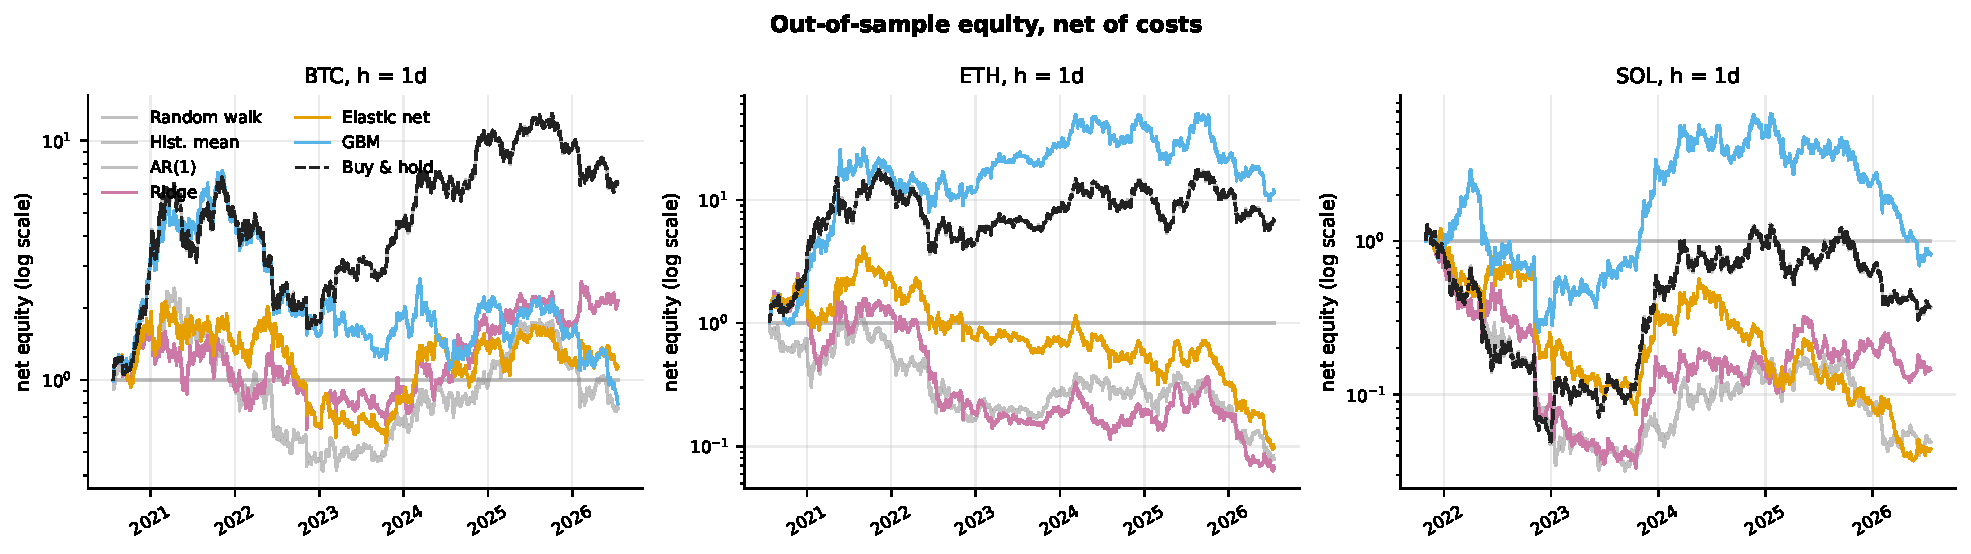
\includegraphics[width=\linewidth]{fig6_equity.pdf}
  \caption{Out-of-sample equity net of costs at $h=1$, against the always-long
  reference on the same schedule and cost model. Starting capital is unity and the
  vertical scale is logarithmic.}
  \label{fig:equity}
\end{figure}

\end{document}
